%%%%%%%%%%%%%%%%%%%%%%%%%%%%%%%%%%%%%%%%%%%%%%%%%%%%%%%%%%%%%%%%%%%%%%%%%%%%%%%%%%%%
%Do not alter this block of commands.  If you're proficient at LaTeX, you may include additional packages, create macros, etc. immediately below this block of commands, but make sure to NOT alter the header, margin, and comment settings here. 
\documentclass[12pt]{article}
 \usepackage[margin=1in]{geometry} 
\usepackage{amsmath,amsthm,amssymb,amsfonts, enumitem, fancyhdr, color, hyperref,comment, graphicx, environ,mathtools, bbm, tikz, setspace, cleveref,listings, dcolumn}
\usepackage{array, multirow, caption, booktabs}
\usepackage{ mathrsfs }
\usetikzlibrary{matrix,positioning}
\tikzset{bullet/.style={circle,draw=black,inner sep=8pt}}
\DeclareMathOperator*{\argmax}{arg\,max}
\DeclareMathOperator*{\argmin}{arg\,min}
\DeclareMathOperator*{\Var}{\text{Var}}
\DeclareMathOperator*{\Cov}{\text{Cov}}

\DeclarePairedDelimiter\norm{\lVert}{\rVert}%
\newtheorem{theorem}{Theorem}
\newtheorem{lemma}[theorem]{Lemma}
\DeclareMathOperator{\eps}{\varepsilon}
\doublespacing
\DeclarePairedDelimiter\abs{\lvert}{\rvert}%
\pagestyle{fancy}
\setlength{\headheight}{65pt}
\newenvironment{problem}[2][Problem]{\begin{trivlist}
\item[\hskip \labelsep {\bfseries #1}\hskip \labelsep {\bfseries #2.}]}{\end{trivlist}}
\newenvironment{sol}
    {\emph{Solution:}
    }
    {
    \qed
    }


%%%%%%%%%%%%%%%%%%%%%%%%%%%%%%%%%%%%%%%%%%%%%%%%%%%%%%%%%%%%%%%%%%%%%%%%%%%%%%%%%


\usepackage{xcolor}
 
 


%%%%%%%%%%%%%%%%%%%%%%%%%%%%%%%%%%%%%%%%%%%%%

\rhead{Asha Bharadwaj, Caitlin Dutta, John Higgins, Alexis Smith\\Econ 899 \\ 5 October, 2022} 

%%%%%%%%%%%%%%%%%%%%%%%%%%%%%%%%%%%%%%%%%%%%%


%%%%%%%%%%%%%%%%%%%%%%%%%%%%%%%%%%%%%%

\begin{document}

\section{Transition paths}
We have plotted the transition paths below. For reference, the initial steady state values were $K_0^{SS} = 3.360$, $r_0^{SS} = 0.024$, $L_0^{SS} = 0.343$, and $w_0^{SS} = 1.455$. The new steady state values are $K_T^{SS} = 4.626$, $r_T^{SS} = 0.011$, $L_T^{SS} = 0.366$, and $w_T^{SS} = 1.596$. We see that aggregate capital, effective labor supply, and wages increase, whereas the interest rate decreases. The transition paths are plotted below:
\begin{center}
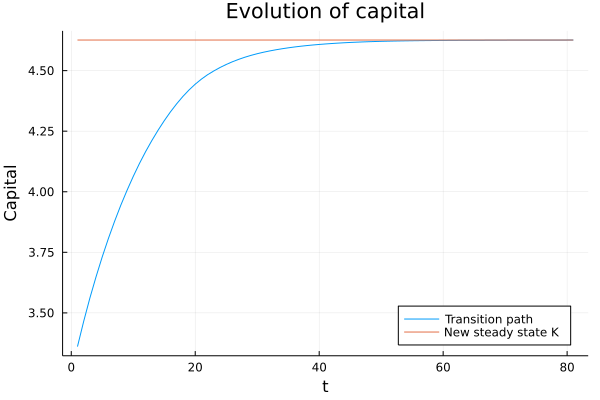
\includegraphics[scale= 0.35]{kplot.png}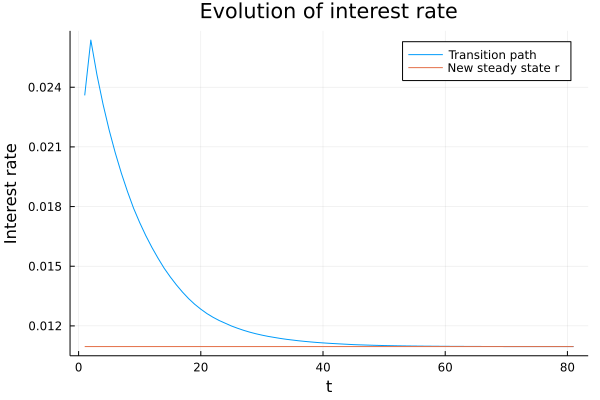
\includegraphics[scale= 0.35]{rplot.png}\\
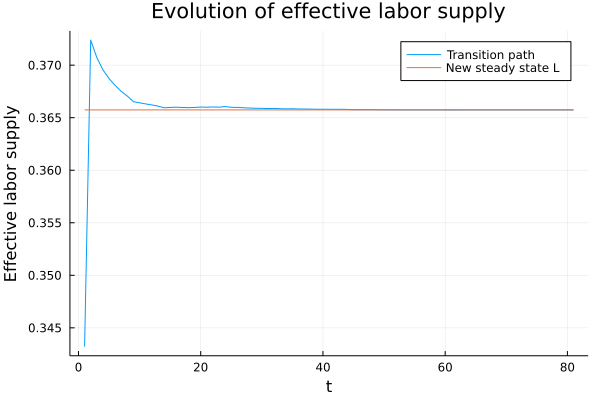
\includegraphics[scale= 0.35]{lplot.png}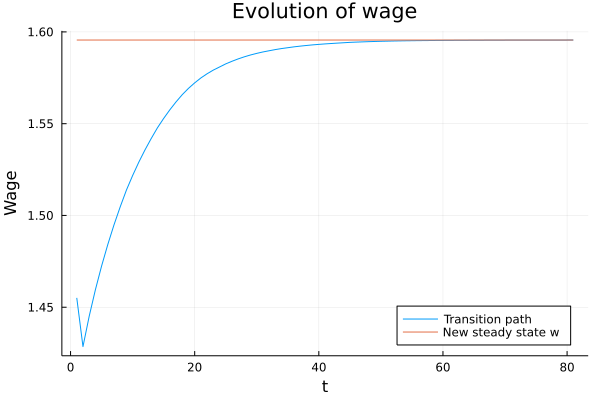
\includegraphics[scale= 0.35]{wplot.png}
\end{center}
We observe the following dynamics. When the policy is announced, people no longer plan on getting benefits in retirement and thus accumulate capital. The incentive to accumulate savings leads them to work more, leading to a sudden uptick in the effective labor supply. As a result, wages initially decrease sharply. 

Furthermore, the sudden spike in labor supply causes an uptick in the interest rate (since the labor supply increases faster than the initial capital increase). This is why the interest rate has an initial spike upwards. However, as the level of capital builds over time, the ratio of capital relative to labor increases and thus the interest rate falls. In turn, as aggregate capital increases, wages fall and so does the labor supply. Over time, each variable converges to its steady state value.

We found that a transition path of length $T = 80$ achieved convergence to the new steady state. The transition paths using $T = 30$ and $T = 50$ both did not get quite close enough to the new steady state values.

\section{Consumption equivalent variation}
We compute the consumption equivalent variation as
\[EV(j, a, z) = \left( \frac{V_0(j, a, z; \theta_0^{SS}, \theta_T^{SS})}{V_0^{SS}(j, a, z; \theta_0^{SS})}\right)^{\frac{1}{\gamma(1-\sigma)}} \]
To find the average across each age group, we compute
\[EV_j = \sum_{z \in Z} \int_{a} EV(j, a, z) \Gamma_0^{SS}(j, a, z; \theta_0^{SS})\, da\]
We plot the measure of EV and the average EV across each age group below:
\begin{center}
    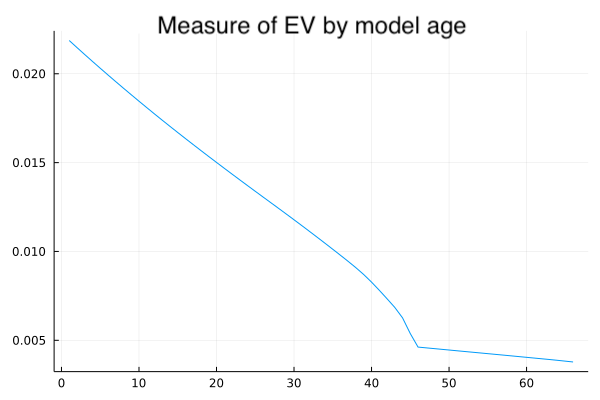
\includegraphics[scale=0.4]{ce_meas.png}\\
    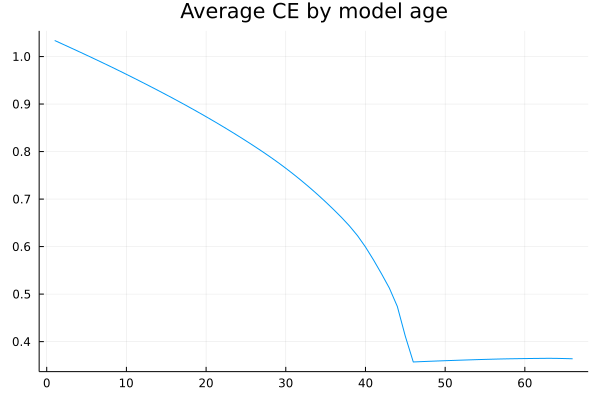
\includegraphics[scale=0.4]{avg_ce.png}
\end{center}
To determine how many people will vote in favor of elimination, we find the mass of agents with $EV(j, a, z) \geq 1$. We find that 11.45\% of the population would vote in favor of social security elimination when taking the transition path into account. As computed in the past homework, the proportion of the population which would vote for social security when the transition path is not taken into account is 16.31\%. Intuitively, the difference between these two is explained by the fact that the transition path doesn't immediately jump to the new steady state level, meaning that the level of capital is less than would be optimal when social security is eliminated. The transition is is in a sense costly: the benefit to the younger workers doesn't accrue until significantly later, which means that on the margin they will be less likely to support. Only the youngest agents (model ages less than 5 or so) would benefit from the transition to the new steady state. 
\section{Impact of future Social Security elimination}
We now repeat the above under the assumption that Social Security benefits are paid through $t= 20$, but that Social Security will be abolished starting in $t = 21$ onward. The important difference is that the elimination is now expected, which allows agents to adjust accordingly. 

We found that it took longer for the economy to get to the new steady state. $T = 50$ did not achieve convergence, whereas $T = 110$ did. The plots of the transition paths are included below:
\begin{center}
    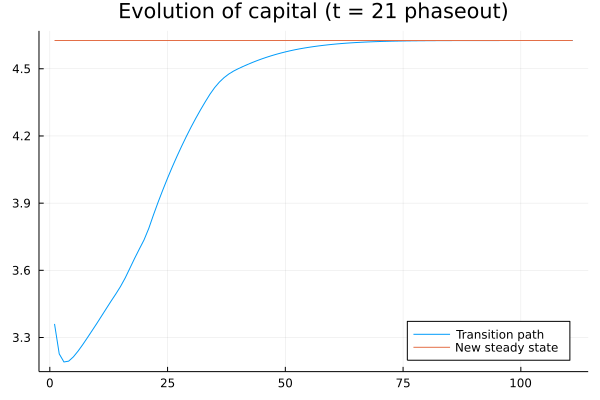
\includegraphics[scale= 0.35]{kplot_21.png}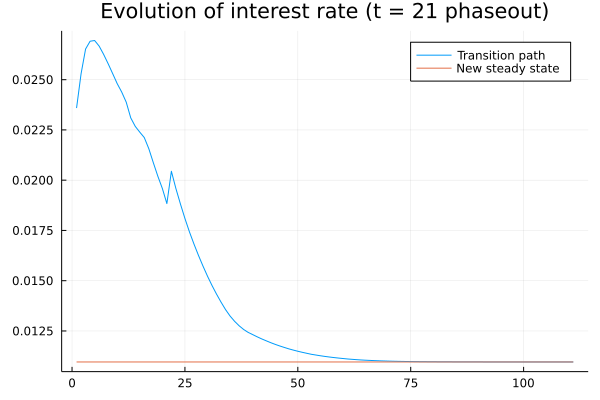
\includegraphics[scale= 0.35]{rplot_21.png}\\
    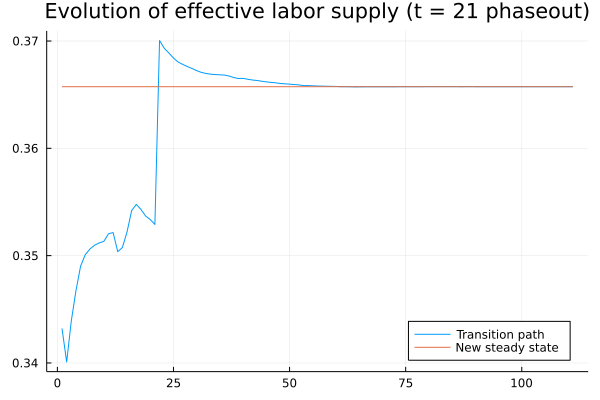
\includegraphics[scale= 0.35]{lplot_21.png}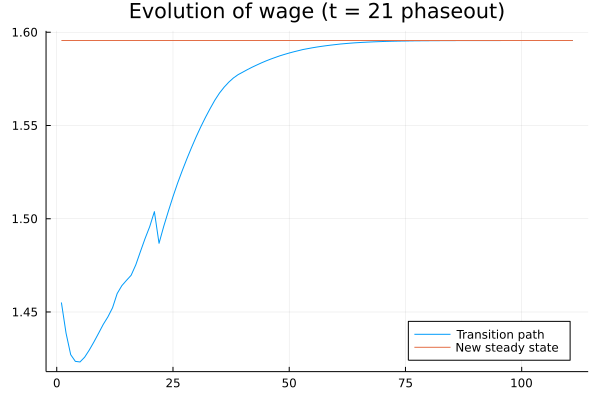
\includegraphics[scale= 0.35]{wplot_21.png}
\end{center}
Overall, similar dynamics are observed as before. However, the jumps that we originally observed at $t = 0$ now occur at $t = 21$ (since this is now when Social Security is eliminated). The level of capital is thus able to converge more gradually to the new steady state, and the labor supply has time to partially increase to the new steady state level before dramatically rising at $t = 21$. 

We plot the mass of consumption EV for each age group as well as the average consumption EV for each age group below:
\begin{center}
    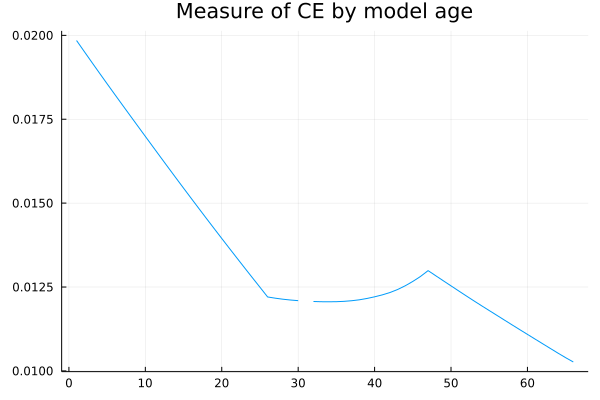
\includegraphics[scale=0.4]{cemeasage_21.png}
    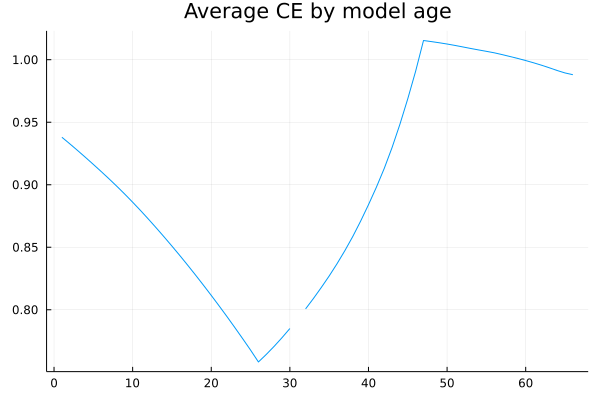
\includegraphics[scale=0.4]{ceavgage_21.png}
\end{center}
(I honestly don't know what happened at age 31 - please mentally interpolate a value)

As before, we can determine the proportion of the population which would vote in favor of elimination at $t = 21$. Roughly 16.38\% of people at time $t=0$ would prefer elimination of Social Security in time $t=21$ when the transition path is taken into account. This is higher than the level of support for elimination at $t=0$. Intuitively, the 20 years before the policy comes into effect give agents time to accumulate the required level of capital once Social Security is phased out. Those who are 20 years out from retirement have 20 years to accumulate savings in preparation for the elimination of social security. This is a stark contrast to the case when it is eliminated at $t=0$, since those agents were planning on having benefits $b$ in retirement and suddenly lost them. 

Mechanically, agents 20 years or more out from retirement choose to work more and save more. This drives up wages and lowers interest rates. However, those closer to retirement don't have to worry as much: they are guaranteed to have benefits for at least part of their retirement. This means they increase their capital holdings more gradually than they would in the case where Social Security was eliminated at $t=0$: they don't need to save as much, meaning that they are able to consume more in the years leading up to retirement than they would if Social Security were immediately eliminated.

However, young agents don't like this as much. They still face 20 years of distortionary labor taxes, yet they don't get any benefits when they retire. The benefit to young agents of eliminating Social Security is in large part due to the elimination of this tax. When eliminated at $t=0$, they are able to increase their labor supply enough (due to the elimination of the wedge) which allows them to save enough to offset the loss of benefits in retirement and increase their current consumption. Phasing out Social Security at $t=21$ doesn't help them, since they pay into the system but they don't get any benefit out of it. 



\end{document}
